\section{Data}\label{app:data}

\subsection{Description of Variables}

\begin{lighttable}[h!]
    \centering
    \footnotesize
    % \caption{Description of Variables}
    \caption*{\scriptsize\emph{Notes:} All variables are defined at the therapeutic class--year level ($i, t$)}
    \vspace{1em}
    \resizebox{\textwidth}{!}{
        \input{tables/description-of-variables}
    }
    \label{app:description-of-variables}
    \vspace{1em}
\end{lighttable}


\subsection{Matching Pharmaprojects to Pitchbook}\label{app:matching_pharma_to_pitch}

We match data on firm founding year and ownership from Pitchbook to Pharmaprojects by firm name. Matching by firm name is challenging, because datasets often use different naming conventions. For example, one dataset may list ``Eli Lilly \& Co.'', while the other simply states ``Lilly''. Here we briefly describe our approach to this inherently noisy matching task and report results from manual validation.

We first filter firms in Pitchbook by their primary industry group, selecting industries that contain the phrases pharmaceuticals, healthcare, drugs, medical, surgical, hospitals, and clinics. We then clean firm names, removing punctuation, special characters, and common legal suffixes, e.g., ltd., inc., co.

Matching on these cleaned firm names produces multiple matches for each firm in Pharmaprojects. For example, we find that Pfizer matches to many subsidiaries or overseas business units. To identify the focal firm in each match, we keep the matched firm with the oldest founding year. If this data is missing, we select the matched firm with the largest number of employees.

Out of 2,804 pharmaceutical firms, we matched 2,150 to Pitchbook. To validate our match, we took a random sample of 50 firms from those that were matched and another random sample of 50 firms from those that were not matched. For those that were matched, we compared the matches across other observable dimensions, such as HQ location. These manual checks revealed one error in the random sample of 50 firms. As for the unmatched firms, we repeated the same process but with the unfiltered Pitchbook data (i.e., not conditioning on pharmaceutical-relevant firms). For the 654 unmatched firms, we found a match for 76 firms. However, we found that only half of these were accurate upon manual inspection.

In sum, our matching approach is highly accurate, but the main limitation is the coverage of the data.

\subsection{Identifying ATC-1 groups}\label{app:indentify_atc1}

In our analyses, we control for unobserved time and industry varying trends using $ATC1\times{Year}$ fixed effects \citep{branstetter2022generic}. Our data, however, do not include the ATC-1 code to which the therapeutic class belongs. Fortunately, there are only 14 ATC-1 categories (\url{https://www.who.int/tools/atc-ddd-toolkit/atc-classification}). We exclude ATC P: Antiparasitic products, insecticides and repellents, which leaves 13 codes. In a similar approach to matching our sample to GWAS, we loop through our 200 therapeutic class names and use GPT-4.0 to identify the closest ATC-1 match. We match 139 out of 200 therapeutic class designations to an ATC-1 code. Importantly, the therapeutic classes which we match are those pervasive, as we only lose 268 (out of 2,791) observations when we exclude therapeutic classes that we are unable to match to an ATC-1. We ran all of our analyses including these 268 observations grouped under a pseudonym ATC-1 `X'. Though not reported here, all of these results were very similar to those reported in the main paper and this Appendix.

\subsection{Matching Pharmaprojects to GWAS}\label{app:matching_pharma_to_gwas}

%\todo[inline]{GWAS is only for diseases due to genetic mutations - though that might be the bulk of the diseases}

A key feature of our analysis includes controlling for the frequency of discovery. The variable we construct---$\ln$(Discovery)---is the natural logarithm of the number of GWAS publications reporting a new target relevant to therapeutic class $i$ in year $t$. 

Founded in 2008 by the National Human Genome Research Institute, GWAS (\url{https://www.ebi.ac.uk/gwas})---or the Catalog of human Genome-Wide Association Studies---is a record of all scientific publications in top-tier journals reporting the discovery of a new target--disease correspondence. An in-depth overview of GWAS is provided by \citet{tranchero2023finding}. 

\begin{lightfigure}[h!]
\caption{\textsc{New Gene-Disease Discoveries Over Time}}
\label{fig:discovery_over_time}
    \centering
        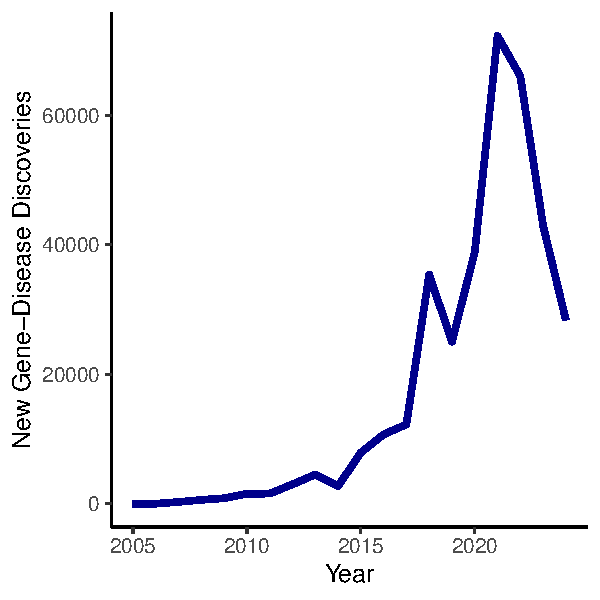
\includegraphics[width=.4\linewidth]{figures/discovery_over_time.pdf}
\end{lightfigure}

The GWAS catalog only reports the disease and/or trait that a particular study is concerned with, so to match these data to Pharmaprojects, we need to make a correspondence between disease/traits and therapeutic class. We create two lists of the 200 distinct therapeutic class names and 28,540 disease names from GWAS. We then wrote a Python script that looped through each disease name and used OpenAI's GPT-4.0 API to identify any and all (at most three) corresponding therapeutic class names. We matched 22,381/28,840 disease names to 179/200 therapeutic classes. Then, for each therapeutic class--year, we count the number of new discoveries in corresponding diseases published in GWAS in that year. As Figure \ref{fig:discovery_over_time} shows, the coverage of GWAS is considerably weaker for the first three-quarters of our sample period (GWAS was only founded in 2008, after all). Consequently, we have a measure of discovery for 811 out of 2791 market observations. After dropping observations where we don't have an ATC-1 code, this becomes 809. 
